\chapter{控制系统脆弱性量化评估体系}
\label{cha:Design}
\section{引言}
\label{sec:chap4:int}
通过前文对控制系统脆弱性概念的定义及深入研究,已明确了控制系统稳定性、可靠性、鲁棒性与脆弱性概念的区别与联系,并结合控制系统鲁棒稳定性的相关概念来分析控制系统的脆弱性。

在前一章中,通过对实际物理系统加性不确定环节的抽象分析,根据物理系统随工作环境改变参数的变化,分析了控制系统在不同工作环境中的鲁棒稳定裕度,得到了鲁棒稳定裕度变化曲线。由于控制系统的脆弱性概念具有主观性,单纯通过鲁棒稳定裕度的变化曲线来量化分析控制系统的脆弱性存在着诸多困难,难以得到脆弱性的量化结果。

为了进一步量化分析控制系统的脆弱性,得到脆弱性量化评价结果,在本章中将脆弱性量化分析问题定位为多指标综合评价问题。针对所得到的鲁棒稳定裕度变化曲线,根据脆弱性的定义与特征选取能够反映系统脆弱现象的评价指标,结合综合评价法及多指标融合法,建立了控制系统脆弱性量化评估的数学模型。解决了控制系统脆弱性现象难以量化的问题,为后续分析空间电源系统脆弱性问题奠定了理论基础。
\section{控制系统脆弱性量化评估指标与数学描述}
\label{sec:chap4:Fragility_Mathdiscribe}
为综合评价系统鲁棒稳定裕度变化曲线所反映的系统脆弱性现象,需要选择能够真实反映系统脆弱性的评判指标,并对各指标进行归一化处理与指标权重分配,建立脆弱性量化评估体系,最终得到一个在~$0\sim1$~范围内的系统脆弱性综合评估结果。
%\newpage
\subsection{控制系统脆弱性量化指标的选取}
\label{sub:chap4:Fragility_Index}
 ~(1)~脆弱性指标一~:

脆弱性反映的基本问题是在工作环境发生剧烈变化时,系统抵御不确定性能力的变化程度。根据第二章空间电源极端工作环境的分析,工作环境的变化可以具体化为极端辐射环境中温度的变化,对空间电源系统的影响体现在电子元器件的数学模型上。为评估在环境变化过程中系统受到的整体影响,第一个脆弱性指标选为在环境温度变化范围内,系统鲁棒稳定裕度的最大值~$\gamma_{max}$~与最小值~$\gamma_{min}$~的差值与温度变化量~$\Delta T$~的比值,即
\begin{equation}\label{equ:chap4:Index1}
  Index_1=\frac{\gamma_{max}-\gamma_{min}}{\Delta T}
\end{equation}

 ~(2)~脆弱性指标二~:

控制系统鲁棒稳定裕度曲线在工作环境变化过程中的波动范围是系统脆弱性的重要表征之一。若系统鲁棒稳定裕度在工作环境变化过程中一直保持在理想值~$\gamma_{E}$~周围小幅度波动,则说明系统在环境变化过程中具有较好的鲁棒稳定裕度,即系统不表现为脆弱特性。若控制系统的鲁棒稳定裕度大幅度偏离理想值~$\gamma_{E}$,则说明在工作环境大幅度变化过程中系统经常要在较差的鲁棒稳定裕度指标下工作。这种控制系统在工作中易受到不确定性的影响,容易产生工作不稳定的情况,即系统表现为脆弱特征。

为了量化反映控制系统鲁棒稳定裕度变化曲线的波动范围,评估如图~\ref{fig:chap4:fig4.1}~所示差值~$\gamma_{max}-\gamma_{min}$~相同但最大值~$\gamma_{max}$~与最小值~$\gamma_{min}$~不同的曲线~1,2~以及如图~\ref{fig:chap4:fig4.2}~所示差值~$\gamma_{max}-\gamma_{min}$、最大值~$\gamma_{max}$~与最小值~$\gamma_{min}$~相同,但变化趋势不同的曲线~3,4,第二个脆弱性量化评价指标通过比较系统鲁棒稳定裕度均值~$\bar{\gamma}$~与理想指标~$\gamma_E$~并将差值与理想指标相比,量化反映系统鲁棒稳定裕度值与理想值的偏差。根据第三章中系统鲁棒稳定裕度的分析,最理想的鲁棒稳定裕度值应为~1,即不确定性对系统造成的影响为~0,则脆弱性指标二由式~\ref{equ:chap4:Index2}~所示。
\begin{equation}\label{equ:chap4:Index2}
  Index_2=\frac{\left|\bar{\gamma}-\gamma_E \right|}{\gamma_E}=\left|1-\bar{\gamma}\right|
\end{equation}
%\newpage
\begin{figure}[htb]
\centering
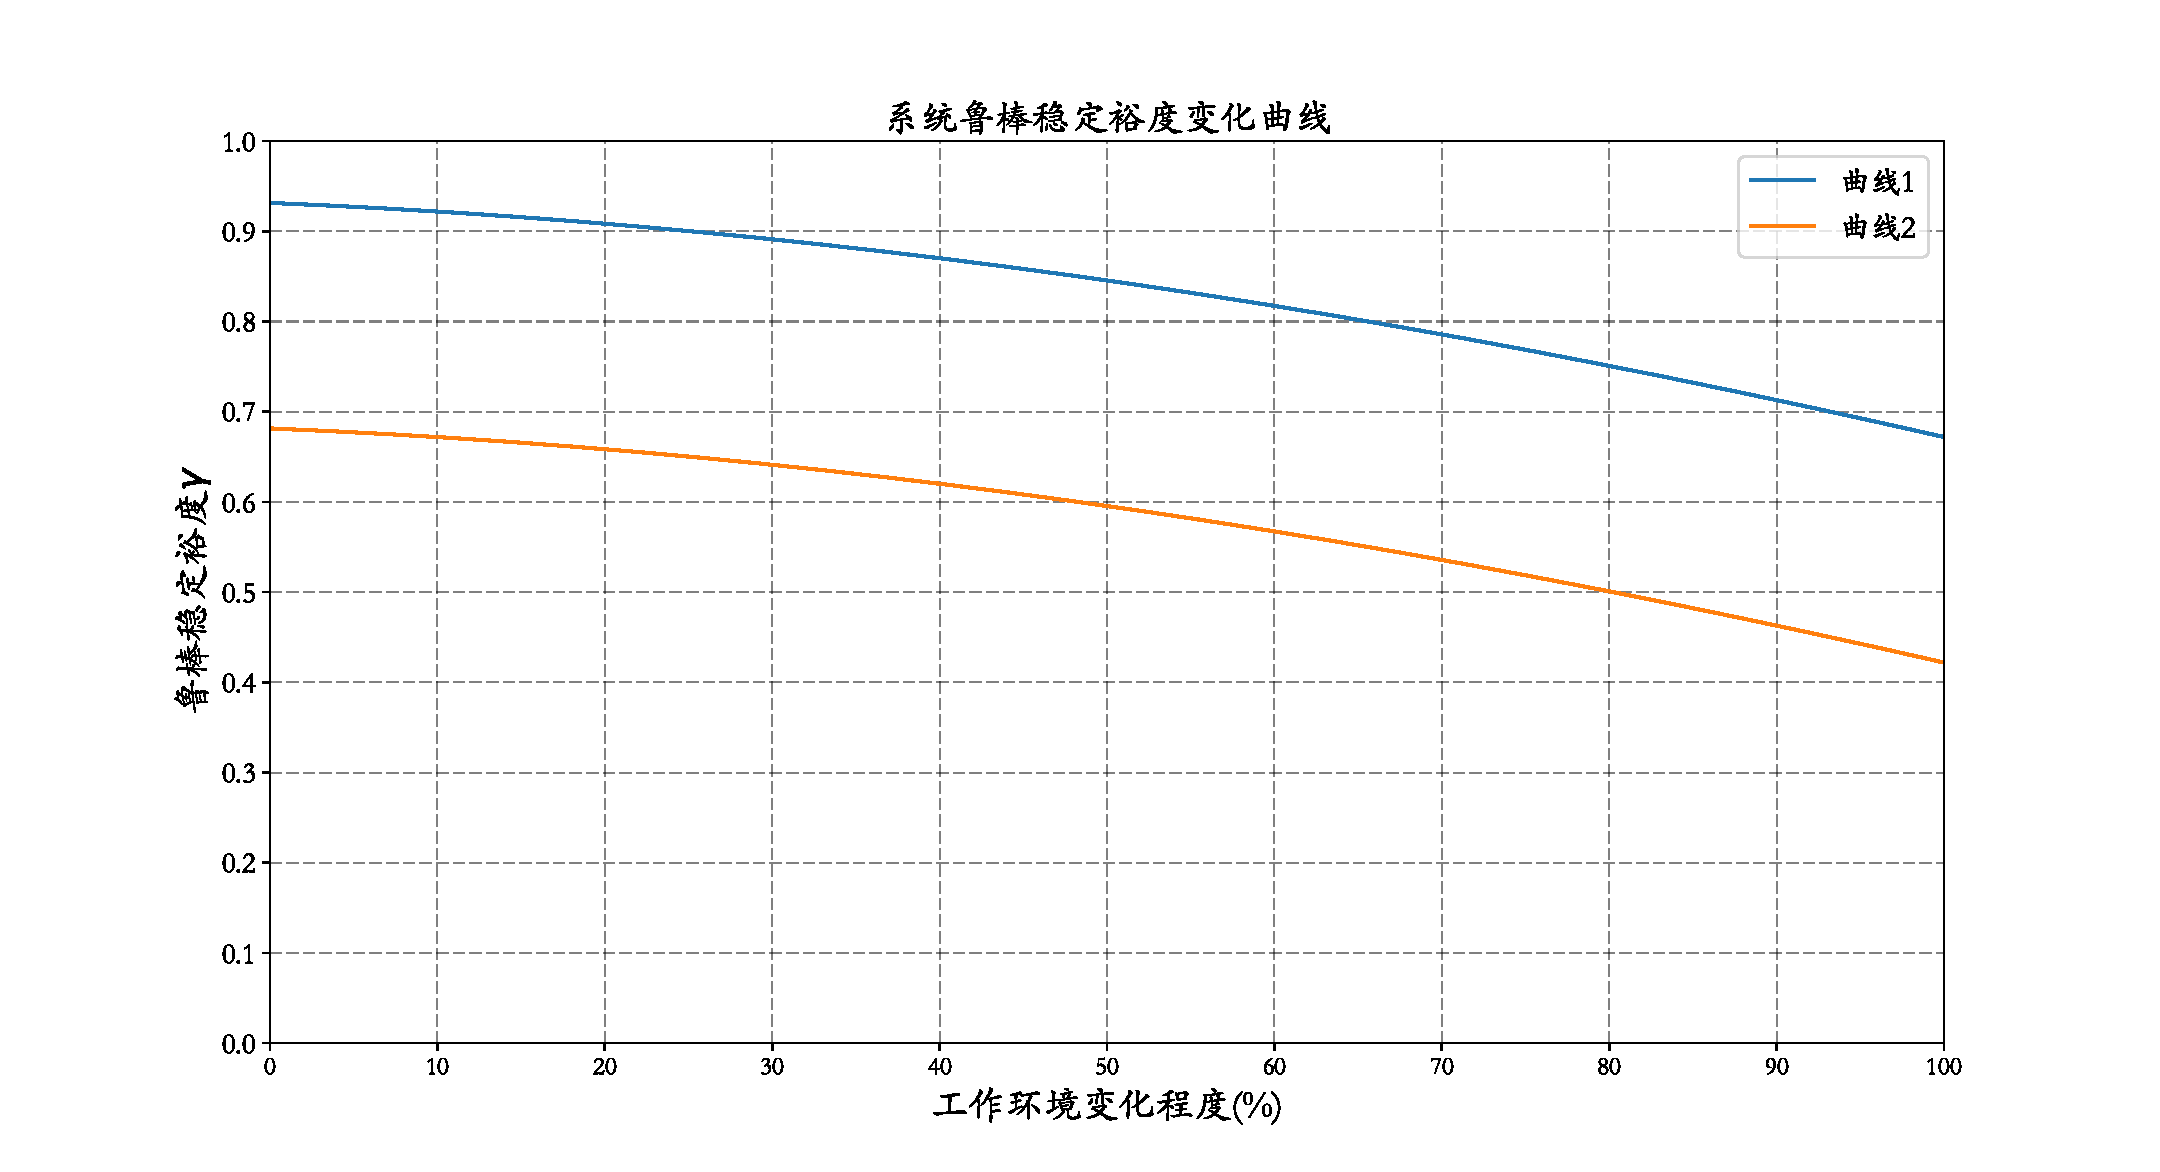
\includegraphics[width=12.5cm]{figure1.pdf}
\caption{鲁棒稳定曲线趋势一}\label{fig:chap4:fig4.1}
\end{figure}
\begin{figure}[htb]
\centering
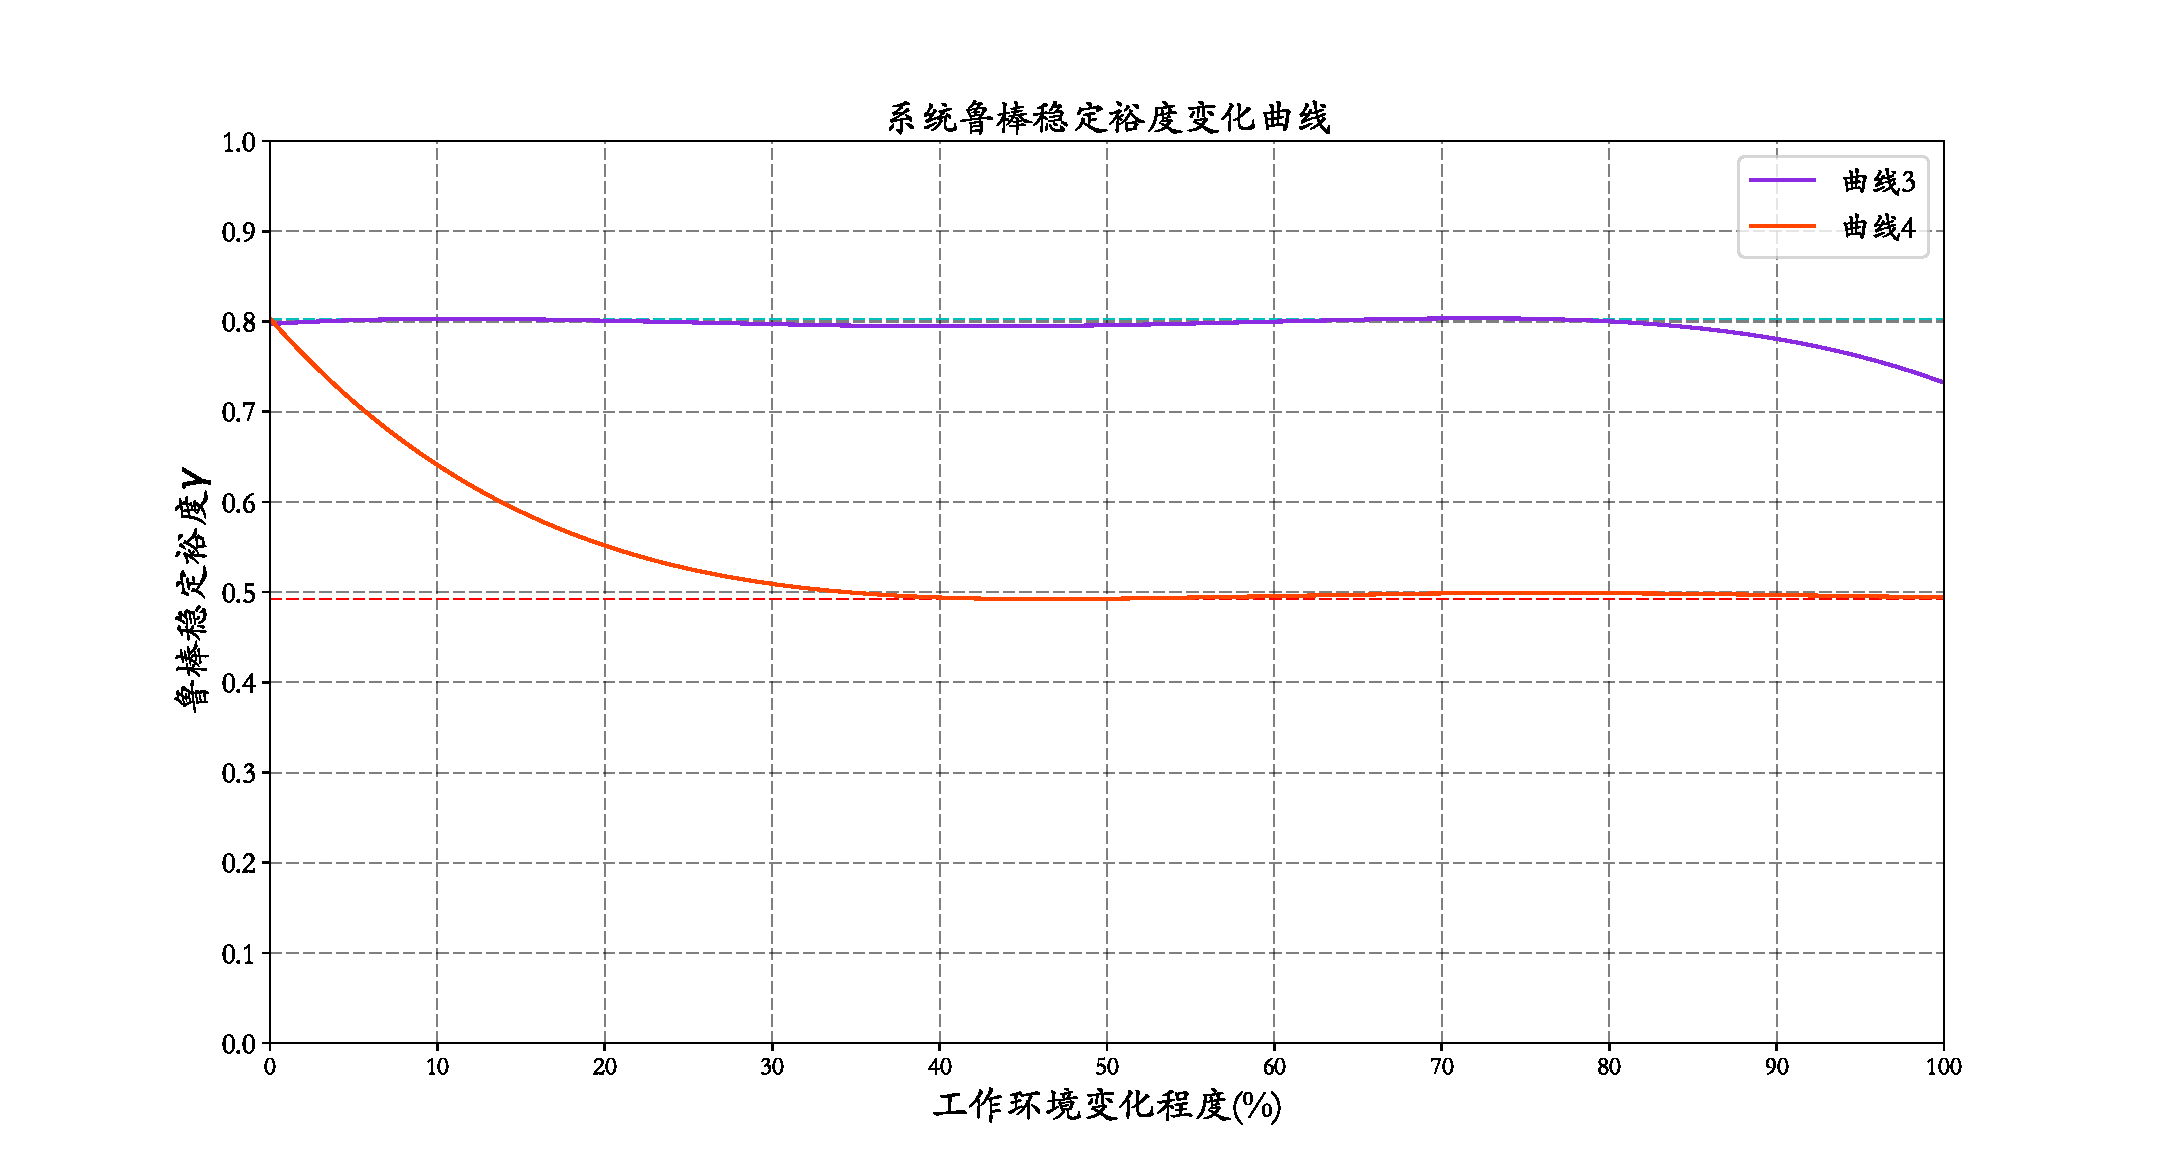
\includegraphics[width=12.5cm]{curve6-7.pdf}
\caption{鲁棒稳定曲线趋势二}\label{fig:chap4:fig4.2}
\end{figure}
\newpage
~(3)~脆弱性指标三~:

为量化评估如图~\ref{fig:chap4:fig4.3}~所示的鲁棒稳定裕度差值~$\gamma_{max}-\gamma_{min}$~相同,最大值~$\gamma_ {max}$~与最小值~$\gamma_{min}$~相同,但变化走势不同的曲线~2~与曲线~5,第三个脆弱性指标选择曲线变化率的最大值。由于实际系统工作时,工作环境的变化趋势无法确定,因此选择曲线斜率绝对值的最大值作为第三个脆弱性指标。

对不同工作环境中系统的鲁棒稳定裕度数据进行多项式拟合,得到鲁棒稳定裕度曲线的多项式表达式。再对该多项式进行求导,取得求导后多项式绝对值的最大值,表征鲁棒稳定裕度曲线的最大变化率。
\begin{figure}[h]
\centering
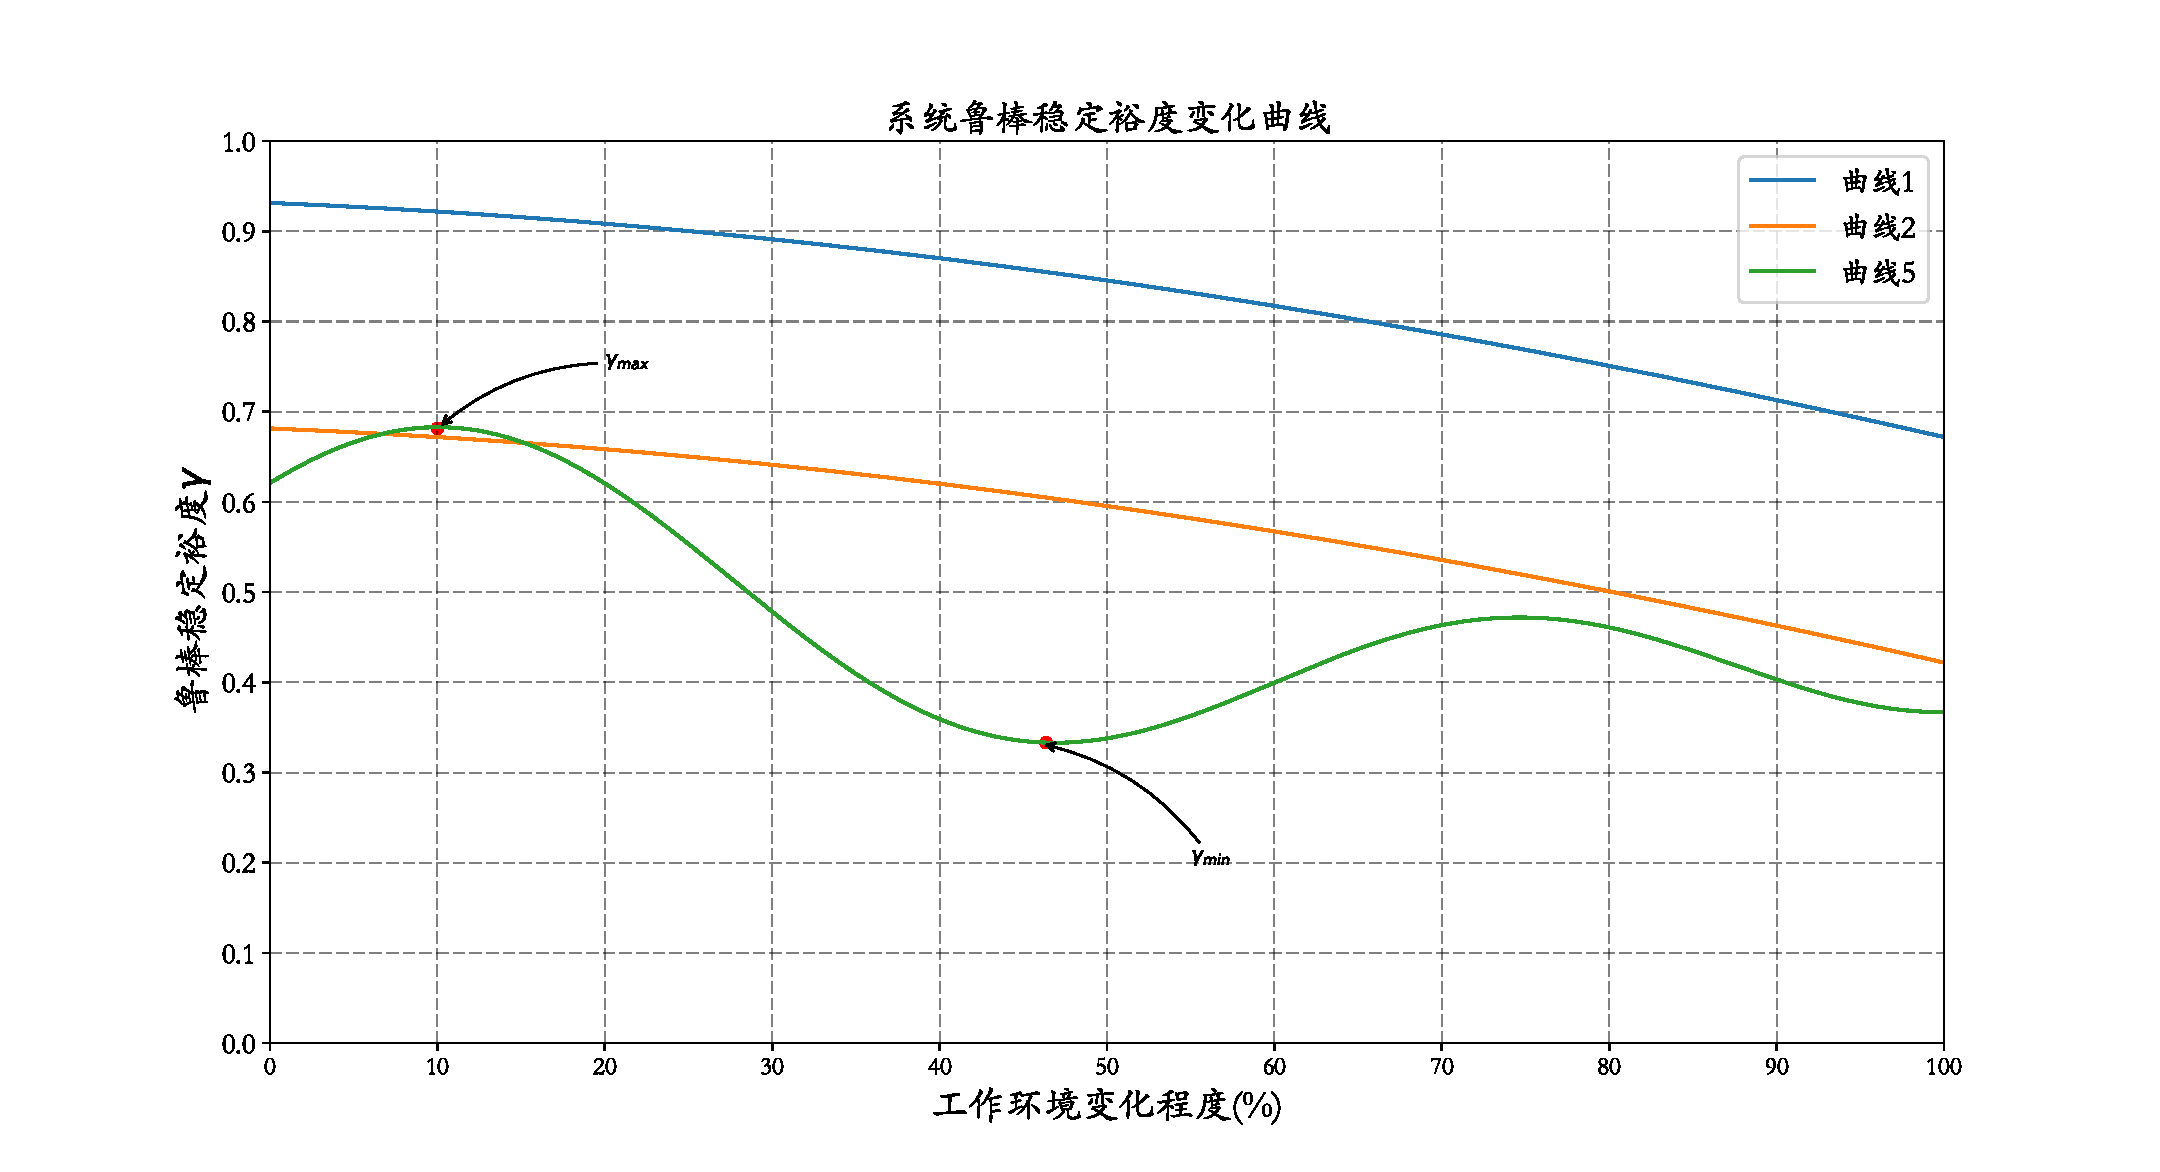
\includegraphics[width=12.5cm]{figure3.pdf}
\caption{鲁棒稳定曲线趋势三}
\label{fig:chap4:fig4.3}
\end{figure}

为避免通过多项式拟合得到的系统鲁棒稳定裕度曲线斜率出现无穷大现象,科学地设置第三个脆弱性量化评价指标的上限阈值。当多项式拟合的鲁棒稳定裕度曲线出现突变的情况,即导数出现无穷大时,脆弱性量化评价指标三取上限值,脆弱性指标三由式~\ref{equ:chap4:Index3}~所示。
\begin{equation}\label{equ:chap4:Index3}
  Index_3=\left\vert\frac{d\gamma}{dT}\right\vert_{max}
\end{equation}

~(4)~脆弱性指标四~:

为量化评估鲁棒稳定裕度差值~$\gamma_{max}-\gamma_{min}$~相同,最大值~$\gamma_{max}$~与最小值~$\gamma_{min}$~相同,但波动频率不同的曲线,本文将系统鲁棒稳定裕度曲线上下波动的次数作为第四个脆弱性量化评估指标。如图~\ref{fig:chap4:fig4.4}~所示,虽然曲线~6~与曲线~7~波动幅度相同,但曲线~6~相比曲线~7~的波动次数明显更少,即曲线~6~对应的系统鲁棒稳定裕度性能更为稳定。
\begin{figure}[h]
\centering
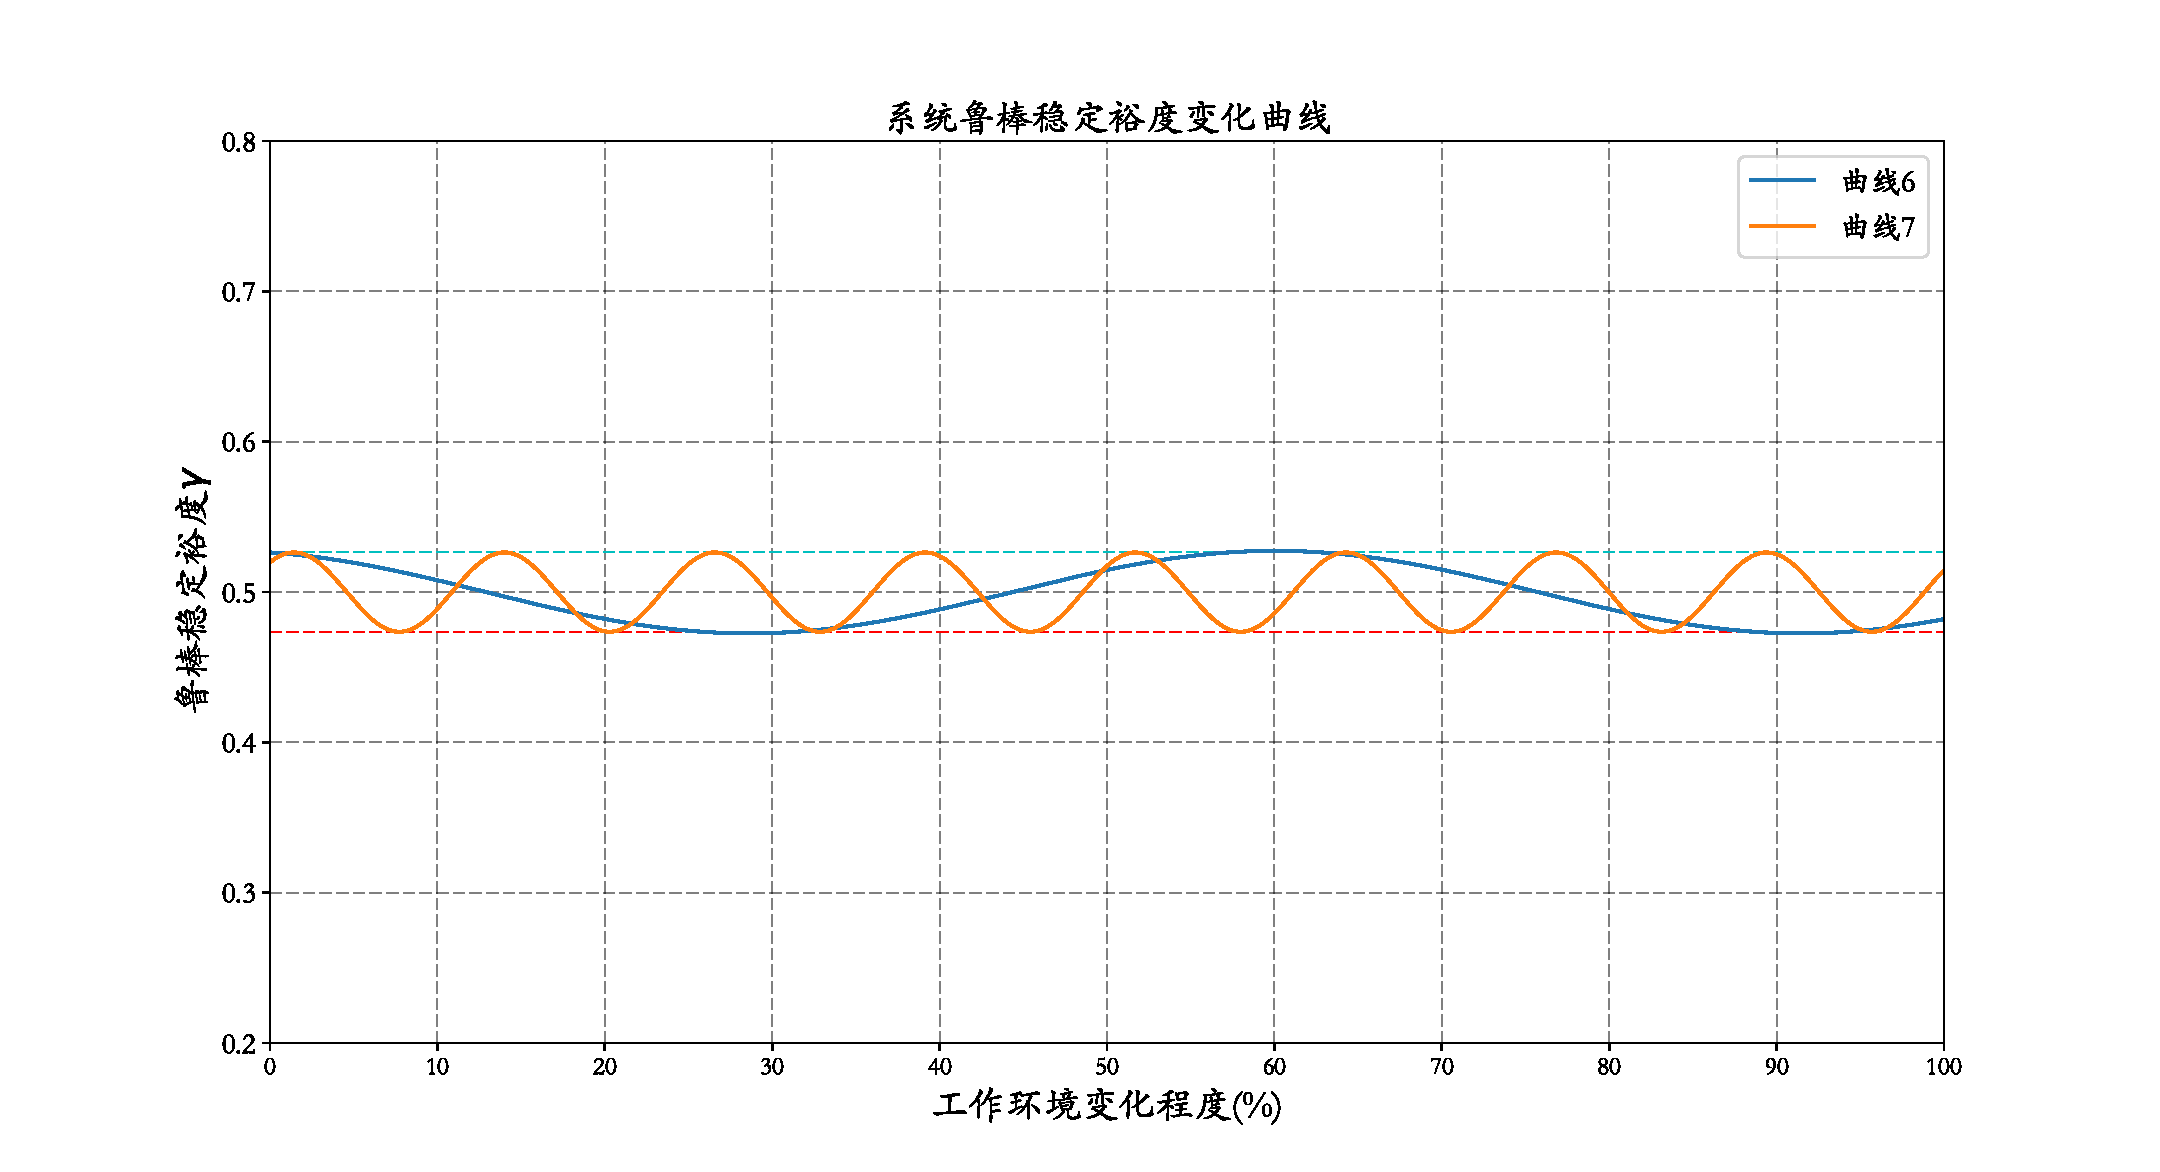
\includegraphics[width=12.5cm]{figure2.pdf}
\caption{鲁棒稳定曲线趋势四}
\label{fig:chap4:fig4.4}
\end{figure}

因此,考虑对拟合得到的系统鲁棒稳定裕度变化曲线多项式表达式求导,计算求导后多项式的零点个数,作为第四个脆弱性评价指标。
\begin{equation}\label{equ:chap4:Index4}
  Index_4=\left(n_{zero}\right)\vert_{\frac{d\gamma}{dT}}
\end{equation}

通过对控制系统鲁棒稳定裕度曲线变化趋势的分析,选取了四个能够反映系统脆弱性现象的评价指标,作为控制系统脆弱性量化评估的依据。未经归一化的控制系统脆弱性量化评价指标向量~$IND_0$~为
\begin{equation}\label{equ:chap4:Index5}
  IND_0=\left[~Index_1~~~Index_2~~~Index_3~~~Index_4~\right]
\end{equation}
\subsection{脆弱性量化评估指标的语义分析}
\label{sub:chap4:Fragility_semantic}
脆弱性指标一表征系统在工作环境发生大幅度变化时,系统抵御不确定性能力的变化程度。若在整个环境变化过程中,抵御不确定性能力的鲁棒稳定裕度指标变化较小,则说明系统脆弱性越好,即系统不脆弱。

脆弱性指标二表征系统鲁棒稳定裕度均值与理想指标的偏差程度。若偏差值越小,代表系统鲁棒稳定裕度值在理想指标附近浮动,系统鲁棒稳定裕度接近理想值,即系统脆弱性越好。

脆弱性指标三表征系统鲁棒稳定裕度曲线最大的变化率。若鲁棒稳定裕度曲线存在较大的变化率,则表征系统鲁棒稳定裕度曲线存在向上或向下突变的情况,即鲁棒稳定裕度值快速变差,系统脆弱性差。若系统鲁棒稳定裕度曲线不存在快速变化的情况,即指标三的值较小,则系统脆弱性好。

脆弱性指标四表征系统鲁棒稳定裕度曲线在环境变化过程中波动的情况。脆弱性好的系统,其鲁棒稳定裕度曲线在工作环境变化的过程中不存在较多的波动,一直保持着在理想指标附近。若鲁棒稳定裕度曲线存在较多次上下波动,即指标四的值较大时,系统脆弱性较差。系统脆弱性指标四的值越小表征系统脆弱性越好。

因此,综合分析以上四个指标所对应的系统本质特性,以及在数学描述上
指标值与语义分析的统一性可知,由以上四个指标所组成的系统脆弱性综合指标越小,系统脆弱性越好,即系统不脆弱;系统的综合脆弱性指标越大,系统脆弱性越差,即系统越脆弱,与实际语义相符。
\section{脆弱性量化评估指标归一化数据处理}
\label{sec:chap4:Fragility_DataAnalysis}
由上述分析可知,系统的各个脆弱性评价指标代表的是系统鲁棒稳定裕度曲线的不同属性,反应的是系统脆弱性现象的不同特征,每个指标的数量级都是不同的。因此,需要将这五个指标进行归一化处理,将数据统一映射到~[0,~1]~区间上,消除数量级的差异,从而将五个指标进行加权处理得到系统的综合脆弱性量化评估结果。
\subsection{脆弱性量化指标归一化方法确定}
不同的数据格式及应用模型要求对数据采用不同的归一化方法,从而对特定的应用模型得到良好的数据分析效果。数据归一化的方法多种多样,常用的数据归一化方法见表~\ref{tab:chap4:normalize}。
\newpage
\begin{center} \tablecaption{常用的数据归一化方法 \label{tab:chap4:normalize}}
\tablefirsthead{
\bottomrule
\multicolumn{1}{c}{T$\left(^{\circ}C\right)$} &
\multicolumn{1}{c}{ $\gamma_C$}  &
\multicolumn{1}{c}{ $\gamma_L$}  &
\multicolumn{1}{c}{ $\gamma_R$} \\}
\tablehead{\multicolumn{2}{c}{
\small 续表 \ref{tab:chap5:data}} \\
\bottomrule
\multicolumn{1}{c}{T$\left(^{\circ}C\right)$} &
\multicolumn{1}{c}{ $\gamma_C$}  &
\multicolumn{1}{c}{ $\gamma_L$}  &
\multicolumn{1}{c}{ $\gamma_R$} \\}
\tabletail{\bottomrule
\multicolumn{2}{c}{\small 接下页} \\}
\tablelasttail{\bottomrule}
\begin{supertabular}{C{4cm}C{3cm}C{3cm}C{3cm}}
      \midrule
      %\tabincell{c}{}
        \tabincell{c}{离差标准化\\(Min-max Normalization)}

         & 适用于最大最小值明确不变的数据      & 不改变数据的原始分布      & $x^{\ast}=\FS{x-x_{min}}{x_{max}-x_{min}}$  \\ \\

       z-score~标准化       & 适用于最大值最小值未知的情况,且数据接近正态分布
                                        & 改变数据的原始分布,对离群点规范化效果好            & $x^{\ast}=\FS{x-\mu}{\sigma}$       \\ \\

      Logistic~标准化       & 适用于对长尾分布的数据作分段操作
                                        & 改变数据的分布情况             & $x^{\ast}=\FS{\ln x}{\ln n_{max}}$       \\ \\

      \tabincell{c}{小数定标标准化\\(Decimal scaling)}    & 适用于数据初期探索,不消除数据属性间权重差异
                                       & 不改变数据分布                      & $x^{\ast}=\FS{x}{10j}$       \\ \\

      排序归一化             & 适用于对数据的具体值并不关心,更关心相对排序的数据
                                       & 原始数据变为直线分布            & $x^{\ast}=\FS{x_{rank}}{num_{total}}$       \\ \\

      分段归一化             & 适用于数据分布有明显分段特征的情况
                                       & 不改变分段数据的分布            & 根据不同数据段,采用不用方法       \\ 
\end{supertabular}
\end{center}
\medskip

其中针对评判指标的数据归一化方法主要采用离差标准化法及~z-score~标准化法。在分类、聚类等算法中,经常需要使用表征距离的数据来度量相似性,在主成分分析法~PCA~的计算过程中,需要对大量的数据进行降维,从而来去除数据中的噪声,挖掘数据中的模式。在这类问题中,z-score~数据归一化方式使得经过处理后的数据符合标准的正态分布特性,可以提升分类、聚类、主成分分析等算法模型的收敛速度及模型精度。但对于不涉及到距离度量计算、协方差计算且原始数据不符合高斯分布的时候,使用~z-score~数据归一化方法改变了原数据的分布特性,归一化处理后使得原有数据丢失了相应的信息。

若明确知道数据的上限值和下限值,可以采用离差标准化的数据归一化方式进行数据处理。即不改变原有数据的分布规律,又将原始数据映射到~[0,~1]~数值区间内,消除了数据之间数量级的差异,解决了因量纲及数量级造成的可比性问题。又由于对原始数据的分布规律没有要求,且经过归一化处理后的数据可以进行相互比较与加权组合,使得离差标准化法成为建立综合评价体系时常用的归一化方式。

由于脆弱性量化评价指标在数据分布上不符合标准正态分布特性,且归一化的主要目的是消除指标之间数量级的差异,并不涉及到距离度量计算和协方差计算。因此,本文在脆弱性量化评估系统中选择离差标准化的方法对脆弱性评价指标进行归一化处理。
\subsection{脆弱性量化指标极值分析}
离差标准化的指标归一化方法首先需要确定各指标的上限值和下限值。脆弱性量化的第一个指标表征的是在工作环境变化过程中系统鲁棒稳定裕度的变化幅度,根据第~2~章的分析采用温度由~$-60^ {\circ}C$~到~$280^ {\circ}C$~极端变化表征恶劣工作环境的变化过程。因此在数学描述上脆弱性量化指标一~$Index_1$~的表达式为
\begin{equation}\label{equ:chap4:Index6}
 Index_1=\FS{\gamma_{max}-\gamma_{min}}{\Delta T}=\FS{\gamma_{max}-\gamma_{min}}{340}
\end{equation}

鲁棒稳定裕度的差值~$\gamma_{max}-\gamma_{min}$~最大值为~1,最小值为~0,因此指标一的上限值为~\begin{footnotesize}$\FS{1}{340} $\end{footnotesize},下限值为~0。

指标二表征的是在工作环境变化过程中鲁棒稳定裕度的波动范围与理想指标的偏差,系统鲁棒稳定裕度的理想值~$\gamma_{E}$~为~1。若鲁棒稳定裕度的均值~$\bar{\gamma}$~与理想指标~$\gamma_{E}$~相同,则偏差值~$\left\vert\bar{\gamma}-\gamma_{E}\right\vert$~为~0,指标二取下限值~0。若鲁棒稳定裕度的均值~$\bar{\gamma}$~为最差值~0,则偏差值~$\left\vert\bar{\gamma}-\gamma_{E}\right\vert$~为~$\gamma_E$~等于~1,指标二取上限值~1。

指标三根据曲线的最大变化率来表征系统鲁棒稳定裕度变差的幅度。若曲线没有波动,则曲线斜率的绝对值为~0,指标三取下限值~0。若系统鲁棒稳定裕度值发生突变,曲线快速变化,则斜率的绝对值为无穷大,需要人为设定指标三的上限值。根据~GJB 4041-200(K)~ 航天用电子元器件质量控制要求手册集成电路质量控制一章中的筛选要求\cite{GJB},单片集成电路需在~$150\pm 2^ {\circ}C$~的高温环境中存储~24~小时,并对集成电路的各项数据进行检测。若检测结果符合标准规范,单片集成电路质量顺利经过质量筛选。

根据航天用电子元件质量控制要求手册的筛选规范,航空航天电源电路需要在~$\pm 2^ {\circ}C$~的温度波动范围内进行测试。因此指标三的最坏情况为在~$\pm 2^ {\circ}C$~的温度波动范围内,鲁棒稳定裕度值~$\gamma$~发生突变,由~1~变为~0,指标三的上限值为~0.25。

指标四是根据鲁棒稳定裕度曲线拟合多项式求导后与~x~轴的交点个数来表征曲线的波动程度,鲁棒稳定裕度值的反复波动是系统性能较差的直观表现。若鲁棒稳定裕度曲线在工作环境变化过程中没有波动,则系统不表现为脆弱性,指标四取下限值~0。理论上来说,鲁棒稳定裕度曲线的波动次数可以呈现无穷大的现象。针对实际应用情况,鲁棒稳定裕度曲线的波动次数大于一定值,就可以认定鲁棒稳定裕度反复波动,系统性能较差。在本文的脆弱性量化评价系统中,量化指标四的上限值设置为~10,即鲁棒稳定裕度曲线拟合多项式求导后与~x~轴的交点个数超过~10~个的情况,取指标四的上限值~10~来计算。

综上所述,脆弱性量化指标的上限值和下限值由表~\ref{tab:chap4:limitation}给出。
\begin{table}[htb]
   \centering
   \renewcommand\arraystretch{1.5}
   \caption{脆弱性量化指标的上限值和下限值}
   \label{tab:chap4:limitation}
     \begin{tabular}{|C{4cm}|C{4cm}|C{4cm}|}
\hline
         脆弱性量化指标          & 上限值                       &下限值                   \\
\hline
             脆弱性指标一          & $\FS{1}{340}$         &$0$  \smallskip\\
\hline
             脆弱性指标二          &  $1$                           &$0$  \\
\hline
             脆弱性指标三          &  $0.25$                     &$0$   \\
\hline
             脆弱性指标四          &  $10$                        &$0$   \\
\hline
\end{tabular}
\end{table}
\subsection{脆弱性量化指标归一化处理}
根据~4.3.2~节指标上限值和下限值的分析,采用离差标准化的方式分别对四个脆弱性量化评价指标进行归一化处理,归一化处理的结果如表~\ref{tab:chap4:Normal_result}~所示
\begin{table}[htb]
   \centering
   \renewcommand\arraystretch{1.6}
   \caption{脆弱性量化指标的归一化处理}
   \label{tab:chap4:Normal_result}
     \begin{tabular}{|C{5cm}|p{7cm}|}
\hline
      \tabincell{c}{归一化后的脆弱性量化指标}     &\hspace{2.5cm}数学表达式               \\
\hline
             脆弱性指标一$^{\ast}$    &\hspace{1.8cm}\begin{small}$Index_{1}^{\ast}=340\cdot Index_1$\end{small}    \smallskip\\

\hline
             脆弱性指标二$^{\ast}$    &\hspace{1.8cm}\begin{small}$Index_{2}^{\ast}=Index_2$\end{small}    \\
\hline
             脆弱性指标三$^{\ast}$    &\hspace{1.8cm}\begin{small}$Index_{3}^{\ast}=4\cdot Index_3$ \end{small}    \\
\hline
             脆弱性指标四$^{\ast}$    &\hspace{1.8cm}\begin{small}$Index_{4}^{\ast}=0.1\cdot Index_4$\end{small}   \\
\hline
\end{tabular}
\end{table}

因此,经过归一化的控制系统脆弱性量化评价指标向量~IND~为
\begin{equation}\label{equ:chap4:Index7}
    IND=\left[~Index_1^{\ast}~~~Index_2^{\ast}~~~Index_3^{\ast}~~~Index_4^{\ast}~\right]
\end{equation}
\section{脆弱性量化评估指标权重分配}
\label{sec:chap4:Fragility_Weight}
\subsection{多指标权重理论}
在统计理论和评价体系中,权重是各个评价指标或评价项目重要性的标志,也表示各个指标在总体评价体系中所起到的不同作用。权重的种类很多,不同类别的权重有着不同的数学特点。按照不同的表现形式,权重可分为绝对权重和相对权重。其中相对权重也称为指标的比重,更能反映各个指标在评价过程中起到的作用。

按照不同的形成方式,权重可分为主观权重和客观权重。客观权重是由数据的表现形式和统计指标的合成方式得到的权重,反映了数据的统计规律,这类评价指标权重分配方法主要有统计平均法、层次分析法、网络分析法、模糊评价法等。主观权重是根据评价体系的研究目的和指标的内在含义,通过人为主观地分析、判断来确定各个指标在整体评价体系中的重要程度,这类权重分配法主要有主成分分析法、变异系数法、熵值法等。

\subsection{基于主观评价的指标权重分配}
控制系统的脆弱性量化评估体系是在系统工作环境大幅度变化的情况下,根据系统鲁棒稳定裕度曲线的变化趋势选取特定的脆弱性评判指标来建立的。由于脆弱性评判指标的选取本身不具备统计特性,且各个指标所对应的系统性能变化趋势对于系统脆弱性评判的重要程度具有较大的主观因素,因此控制系统脆弱性多指标量化评估体系是一个基于主观评价的定权重综合评价体系。本文选用层次分析法的相关理论,采用量化处理主观评价权重的方式对控制系统脆弱性评估指标进行权值分配。

\subsection{层次分析法的基本步骤与流程}
层次分析法~(Analytic Hierarchy Process)~简称~AHP,是~20~世纪~70~年代中期由美国运筹学家托马斯·赛蒂~(T. L. Satty)~正式提出,是一种定性和定量相结合的、系统化、层次化的分析方法。采用层次分析法分析问题,通常需要对问题进行以下几个步骤的处理。

~(1)~建立层次结构模型

在对问题进行深入分析的基础上,将有关的各个因素按照不同的属性自上而下地分解为若干层,同一层的因素从属于上一层的因素或对上一层因素有影响,同时又支配下一层的因素或受下一层因素的作用。层次结构模型的层次数与问题的复杂程度及层次化处理程度相关,对于层次数没有限制,但各层中的因素单独拥有的下一层元素通常不超过九个。最上层为目标层,通常只有一个因素,最下层为各决策方案,中间的元素为准则或指标,若指标与准则超过九个,应考虑进一步层次化处理,划分子准则层。通常构建的层次结构模型如图~\ref{fig:chap4:ahp}~所示。
\begin{figure}[h]
\centering
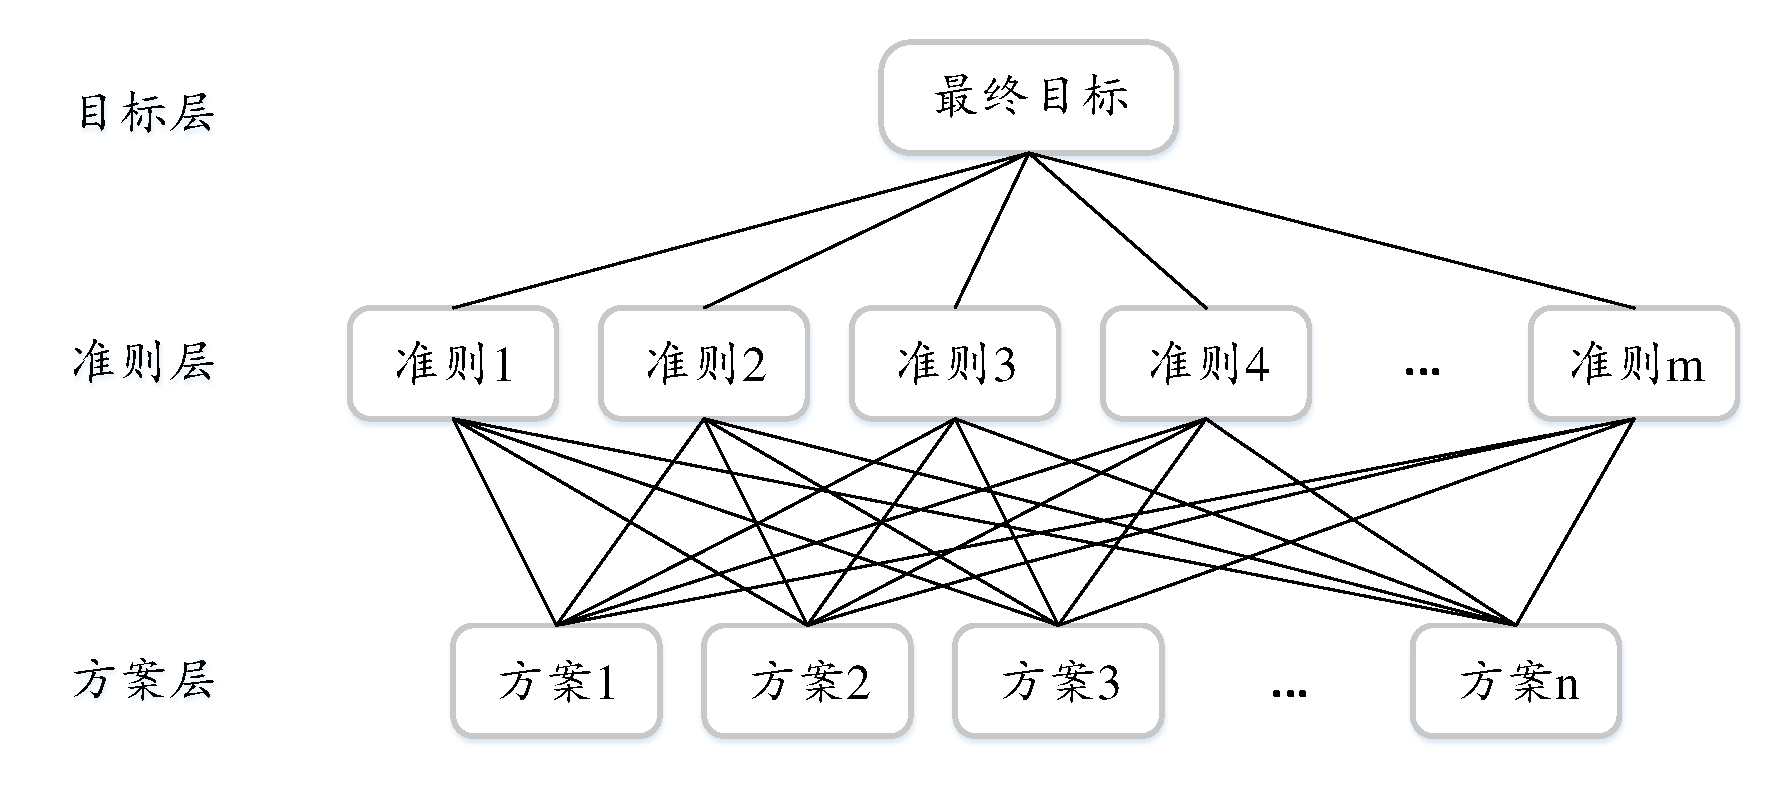
\includegraphics[width=14cm]{AHP.pdf}
\caption{层次结构模型图}\label{fig:chap4:ahp}
\end{figure}

~(2)~构造准则层的判断矩阵

在确定各层各因素之间的权重时,需要将定性的评价指标量化处理,从而构建精确严密的数学模型。构建判断矩阵,将准则层的元素进行两两比较,根据主观定性的评价来度量准则~x~相比于准则~y~的重要程度。采用重要性量化标度~1-9~及其倒数对指标间的相对重要程度进行量化分析。若~x~相对于~y~的标度值大于~1,则表明~x~比~y~重要;若~x~相对于~y~的标度值小于~1,则表明~y~比~x~重要;当且仅当标度值为~1~时,表明~x~与~y~有相同的重要性。通过两两比较的方式,将准则层的相对重要性量化为~1-9~及其倒数,以此作为矩阵元素形成准则层的判断矩阵:

\begin{equation}\label{equ:chap4:Index8}
    A=\left(a_{ij}\right)_{m\times m}
\end{equation}

式中,A~~~为层次分析法某一层的判断矩阵;

\hspace{1.3cm}$a_{ij}$~为因素~i~针对于因素~j~的重要程度标度;

\hspace{1.3cm}m~~为该准则层元素的个数;

判断矩阵~1-9~重要性量化标度定义如表~\ref{tab:chap4:AHP_index}~所示
\newpage
\begin{table}
   \centering
  \renewcommand\arraystretch{1.3}
   \caption{判断矩阵~1-9~重要性量化标度}
   \label{tab:chap4:AHP_index}
     \begin{tabular}{|C{5cm}|C{8cm}|}
\hline
             重要性量化标度               &含义               \\
\hline
             1                                         &表示两个因素相比,前者与后者同等重要   \\
\hline
             3                                         &表示两个因素相比,前者比后者稍显重要  \\
\hline
             5                                         &表示两个因素相比,前者比后者明显重要   \\
\hline
             7                                         &表示两个因素相比,前者比后者强烈重要   \\
\hline
             2,~4,~6,~8                                &表示两个对象相比,前者比后者的重要程度介于上述相邻判断标度之间   \\
\hline
             倒数                                   &若因素~i~相对于因素~j~的重要性为~$a_{ij}$,则因素~j~相对于因素~i~的重要性
                                                           为~$a_{ji}=1\left. \right/a_{ij}$\\
\hline
\end{tabular}
\end{table}

~(3)~判断矩阵的一致性

由于准则层的判断矩阵是通过各因素之间两两比较的重要性得来的,一方面由于客观世界的复杂性和人们认识问题的多样性,另一方面由于~n~个因素两两比较时并没有固定的参数,在进行比较的时候有可能做出一些违反常识的判断,导致采用层次分析法做出的决策不可信。为了保证基于层次分析法的判断意见合理准确,需要检验初始判断矩阵的一致性。

根据矩阵论的相关知识,判断矩阵对应于最大特征值~$\lambda_{max}$~的特征向量经过归一化处理,即为同一层相应元素对应于上一层元素相对重要性的权值排序。由于满足式~\ref{equ:chap4:Index9}~的正互反矩阵被称为一致矩阵。根据定理可知,当且仅当~n~阶判断矩阵最大特征根~$\lambda_{max}=n$~时,判断矩阵为一致。当判断矩阵最大特征根~$\lambda_{max}>n$~时,判断矩阵非一致。 $\lambda_{max}$~比阶数~n~大的越多,判断矩阵的非一致性程度越大。
\begin{equation}\label{equ:chap4:Index9}
    a_{ij}a_{jk}=a_{ik},~~~~\forall i,j,k=1,2,\cdots n
\end{equation}

通常,判断矩阵的阶数越大,其具有完全一致性的难度越大,在层次分析法中虽然不要求判断矩阵完全一致,但要对判断矩阵的一致性满意程度进行度量。为了界定各个阶数判断矩阵的一致性满意度,定义一致性指标~CI~(Consistency Index)~和同阶评价随机一致性指标~RI~之比~CR~(Consistency Ratio)~为随机一致性比例\cite{Deng2012AHP},以此指标度量判断矩阵的一致性满意度。度量判断矩阵一致性的步骤如下~:

1)~计算一致性指标~CI~(Consistency Index)
\begin{equation}\label{equ:chap4:Index10}
    CI=\FS{\lambda_{max}-n}{n-1}
\end{equation}

式中,$\lambda_{max}$~为判断矩阵的最大特征值

\hspace{1.3cm}n~~\quad 为判断矩阵的阶数

2)~查询评价随机一致性指标~RI,如表~\ref{tab:chap4:consistency}~所示
\begin{table}[htb]
   \centering
 %  \renewcommand\arraystretch{1.5}
   \caption{平均随机一致性指标}
   \label{tab:chap4:consistency}
     \begin{tabular}{C{0.5cm}C{0.5cm}C{0.45cm}C{0.45cm}C{0.5cm}C{0.5cm}C{0.5cm}C{0.5cm}C{0.5cm}C{0.5cm}C{0.5cm}C{0.5cm}C{0.5cm}C{0.5cm}C{0.5cm}}
\hline
n     & 1  &2  &3  &4  &5  &6   &7  &8   &9  &10   &11  &12    &13  &14    \\
\hline
RI   &0  &0  &0.52  &0.89  &1.12 &1.24  &1.36  &1.41  &1.46  &1.49   &1.52  &1.54   &1.56  &1.58 \\
\hline
\end{tabular}
\end{table}

3)~计算一致性比例~CR~(Consistency Ratio)
\begin{equation}\label{equ:chap4:Index11}
    CR=\FS{CI}{RI}
\end{equation}

4)~度量判断矩阵的一致性

根据一致性比例~CR~的计算结果,判断矩阵的一致性检测规则如下。

$CR<0.1$~:~说明判断矩阵具有良好的一致性,判断合理;

$CR=0.1$~:~说明判断矩阵具有较好的一致性,判断较为合理;

$CR>0.1$~:~说明判断矩阵不符合一致性原则,需要重新调整,直至满足一致性条件为止。

(4)~权重向量的计算

具有一致性的判断矩阵的最大特征根~$\lambda_{max}$~对应的特征向量经过归一化处理后,可以得到这一层元素对应于上一层元素相对重要性的权重向量。层次分析法中计算权重向量的方法主要有几何平均法~(\ref{equ:chap4:Index12})、算术平均法~(\ref{equ:chap4:Index13})~和特征向量法~(\ref{equ:chap4:Index14})~等。基于以上几种方法可以计算得到比较相近的权重向量,在实际应用过程中可根据需求选取相应合适的权重向量计算方式,得到科学有效的决策结果。
\begin{equation}\label{equ:chap4:Index12}
    W_i=\FS{\left(\prod\limits_{j=1}^{n}a_{ij}\right)^{\frac{1}{n}}}{\sum\limits_{i=1}^{n}\left(\prod\limits_{j=1}^{n}a_{ij}\right)^{\frac{1}{n}}},~~~~i=1,2,\cdots,n
\end{equation}
\begin{equation}\label{equ:chap4:Index13}
    W_i=\FS{1}{n}\sum_{j=1}^{n}\FS{a_{ij}}{\sum_{k=1}^{n}a_{kj}},~~~~i=1,2,\cdots,n
\end{equation}
\begin{equation}\label{equ:chap4:Index14}
    AW=\lambda_{max}W
\end{equation}
\subsection{基于层次分析法的脆弱性评价指标权重分配}
本文所研究的控制系统脆弱性问题,通过分析工作环境变化过程中控制系统鲁棒稳定裕度曲线的变化趋势和特征,建立系统脆弱性量化评估模型。针对已选出的四个评判鲁棒稳定裕度曲线变化趋势和特征的评价指标,采用层次分析法相关理论分配权重。对四个量化评价指标两两比较,依据准则层元素间重要程度~1-9~标度可以得到如表~\ref{tab:chap4:importance}~所示的四项脆弱性评价指标的重要性度量。在重要性度量过程中根据系统脆弱性的定义,指标重要性排序为:指标三~$>$~指标二~$>$~指标一~$>$~指标四。
\begin{table}[htb]
   \centering
 %  \renewcommand\arraystretch{1.5}
   \caption{控制系统脆弱性评价指标重要性度量}
   \label{tab:chap4:importance}
     \begin{tabular}{|C{2cm}|C{2cm}|C{2cm}|C{2cm}|C{2cm}|}
\hline
名称         & 指标一 &指标二                                &指标三                             &指标四                    \\
\hline
指标一     & 1           &$1\left. \right/2$                 &$1\left. \right/3 $             &2                              \\
\hline
指标二     & 2           &1                                          &$1\left. \right/2$              &3                              \\
\hline
指标三     & 3           &2                                          &1                                       &5                              \\
\hline
指标四     &$1\left. \right/2$      &$1\left. \right/3$      &$1\left. \right/5$           &1                              \\
\hline
\end{tabular}
\end{table}

因此,可得控制系统脆弱性评价指标重要性度量初始判断矩阵~$A_0$~为
\begin{equation}\label{equ:chap4:Index15}
\renewcommand\arraystretch{1.5}
 A_0= \left[~~
   \begin{array}{cccc}
     1                        &\FS{1}{2}                         &\FS{1}{3}            &2 \\
     2                        &1                                         &\FS{1}{2}           &3 \\
     3                        &2                                         &1                           &5 \\
     \FS{1}{2}        &\FS{1}{3}                          &\FS{1}{5}            &1
    \end{array}
~~\right]
\end{equation}

利用~MATLAB~软件求解此初始判断矩阵~$A_0$~的特征根及特征向量,采用算术平均法对权重向量进行归一化,得出脆弱性量化评价指标的初始权重分配向量~W为
\begin{equation}\label{equ:chap4:Index16}
    W=\left[~W_1~~W_2~~W_3~~W_4~\right]=\left[~0.1570~~0.2720~~0.4829~~0.0882~\right]
\end{equation}

初始判断矩阵的最大特征根~$\lambda_{max}=4.0145$,根据一致性检验公式计算可知一致性比例为
\begin{equation}\label{equ:chap4:Index17}
    CR=\FS{\lambda_{max}-n}{\left(n-1\right)\cdot RI}=\FS{4.0145-4}{\left(4-1\right)\cdot 0.89}=0.00543
\end{equation}

满足~$CR<0.1$~的一致性检验标准,说明初始判断矩阵具有良好的一致性,判断合理。故初始脆弱性量化评价指标的权重分配向量~W~即为所求,各脆弱性评价指标的权重分配如图~\ref{fig:chap4:chart}~所示。由图可知表征控制系统鲁棒稳定裕度曲线快速变化的指标三权重最大,其对控制系统脆弱性的影响最大。
\begin{figure}[h]
\centering
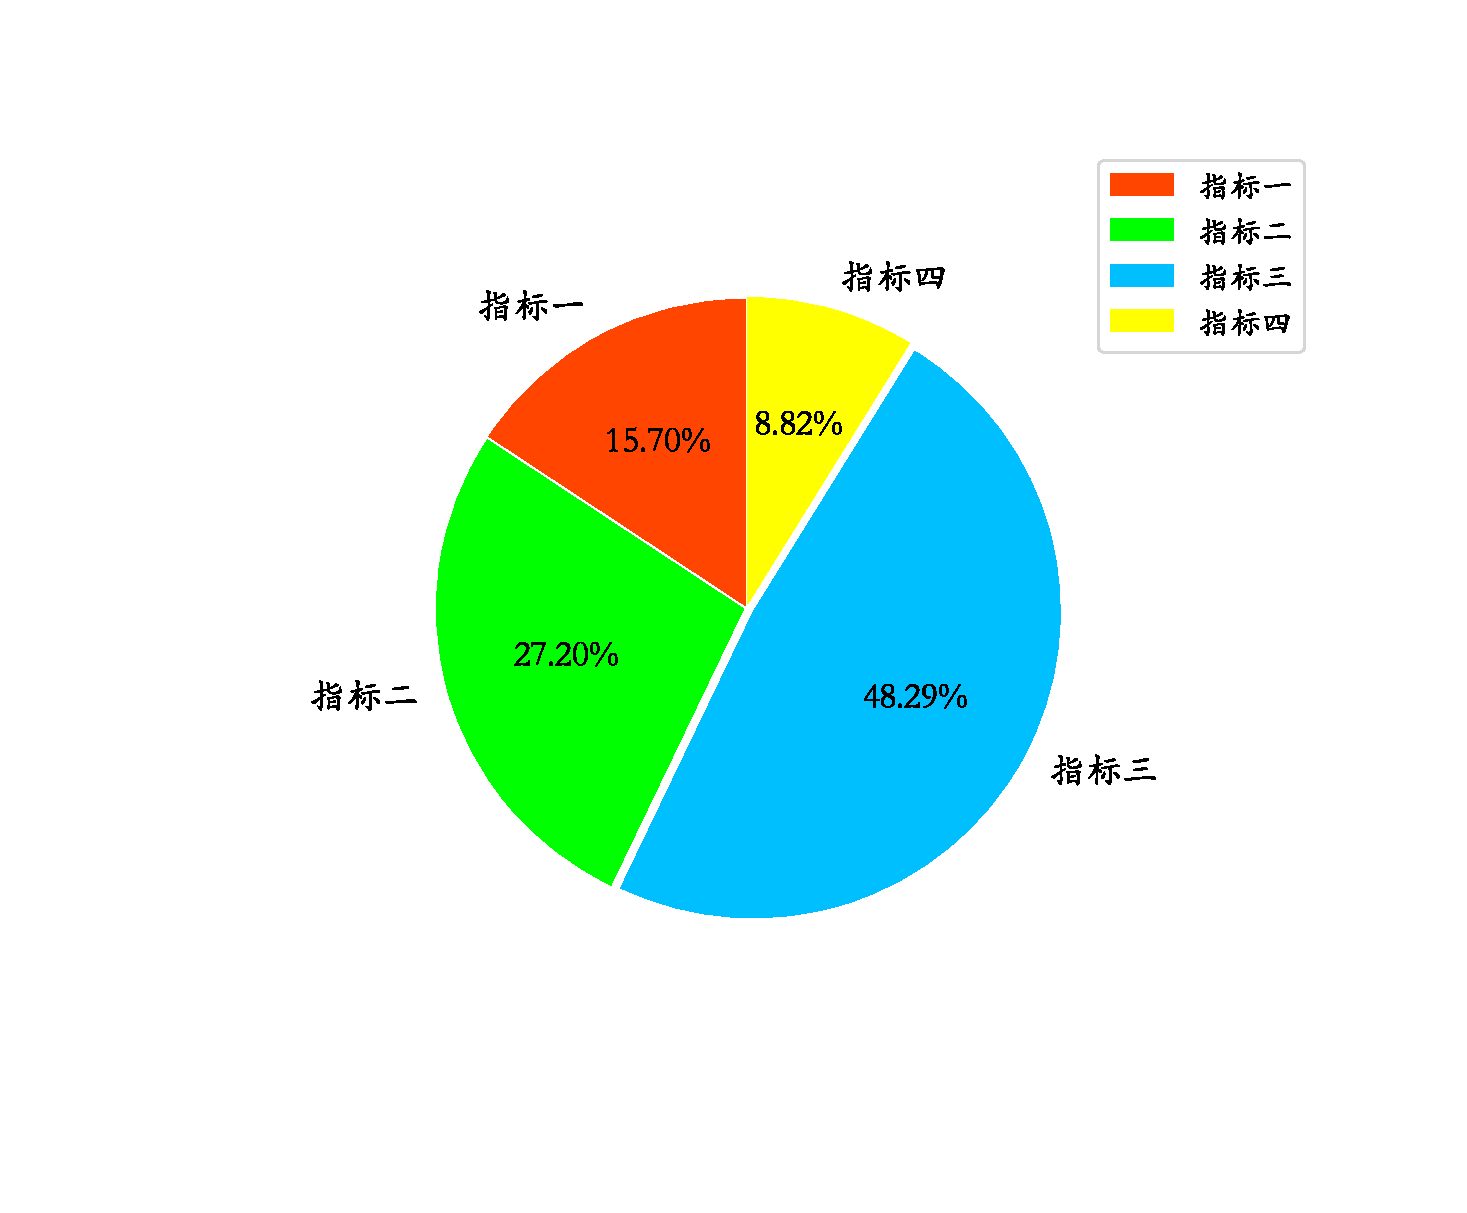
\includegraphics[width=10cm]{Chart.pdf}
\caption{脆弱性评价指标的权重分配}\label{fig:chap4:chart}
\end{figure}
\section{控制系统脆弱性量化评价体系的数学描述}
\label{sec:chap4:Fragility_mathdiscribe}
结合第三章控制系统鲁棒稳定裕度的分析以及上述系统脆弱性指标及权重分配的研究可知,建立控制系统脆弱性量化评价体系的数学模型主要有以下两部分工作。

首先,根据实际控制系统的物理模型及要分析的系统不确定性,将实际控制系统抽象为加性不确定性的系统控制框图。根据实际物理模型工作环境变化时控制系统各环节参数的变化,对系统进行鲁棒稳定性分析,得到系统鲁棒稳定裕度变化曲线。

其次,对所得到的系统鲁棒稳定裕度变化曲线,根据脆弱性的定义分别计算出表征曲线整体变化范围的指标~1、表征曲线均值与理想值偏差的指标~2、表征曲线快速变化程度的指标~3~以及表征曲线反复波动的指标~4,得到未经归一化的控制系统脆弱性量化评价向量~\begin{small}$IND_0=\left[~Index_1~~Index_2~~Index_3~~Index_4~\right]$\end{small}。经过离差标准化归一方法,消除各个指标之间数量级的差别,得到归一化后的控制系统脆弱性量化评价向量~\begin{small}$IND=\left[~Index_1^{\ast}~~Index_2^{\ast}~~Index_3^{\ast}~~Index_4^{\ast}~\right]$\end{small}。采用层次分析法为~4~个脆弱性量化指标进行权重分配,得到权重分配向量~$W=\left[~W_1~~W_2~~W_3~~W_4~\right]$。至此,本文研究的控制系统脆弱性量化评估体系数学模型建立完毕,具体数学描述如~\ref{equ:chap4:Index18}~式所示。
\begin{equation}\label{equ:chap4:Index18}
\begin{split}
    V&=IND\cdot W^T\\
      &=\left[~Index_1^{\ast}~~Index_2^{\ast}~~Index_3^{\ast}~~Index_4^{\ast}~\right]\cdot \left[~W_1~~W_2~~W_3~~W_4~\right]^T,~~V\in \left[0,1\right]
\end{split}
\end{equation}

式中~V~为控制系统脆弱性量化指标,由于各指标及其权重都经过归一化处理,所以脆弱性量化指标~V~的范围为~[0,~1]。由~4.2.2~节进行的指标语义分析可知,4~个脆弱性量化评价指标的值越大,表征系统性能越差,越脆弱。因此作为~4~个评价指标的加权值,脆弱性量化指标~V~的值越大,表征系统越脆弱;脆弱性量化指标~V~的值越小,表征系统越不脆弱。
%%%%%%%%%%%%%%%%%%%%%%%%%%%%%%%%%%%%%%%%%%%%%%%%%%%%%%%%%%%%%%%%%
\section{本章小结}
\label{sec:chap4:sum}
本章通过分析控制系统鲁棒稳定裕度变化曲线,根据脆弱性的定义与特征,选取了~4~个能够反映系统脆弱性现象的评价指标。鉴于系统脆弱性问题的主观性,将控制系统脆弱性量化分析问题定性为一类多指标综合评价问题。结合多指标融合、权重分配及综合评价法的相关理论,对控制系统脆弱性量化评估体系问题进行分析与研究。

首先,对所选出的~4~个脆弱性评价指标进行语义分析,保证~4~个指标在评价系统脆弱性时的统一性、合理性及有效性。然后,根据各指标所表征的实际控制系统性能参数,分析了~4~个指标的上限值和下限值,针对特殊情况人为设置了指标阈值。采用离差标准化法对所选出的~4~个脆弱性评价指标进行归一化操作,消除~4~个评价指标的数量级差异。采用层次分析法将主观的评价与决策量化处理,得到~4~个脆弱性评价指标的权重分配。

最后,结合以上分析、研究的结论,建立了控制系统脆弱性量化评估体系的数学模型,为后续章节中对空间电源电路系统的脆弱性分析与量化评估提供理论方法。